% ВАЖНО
% Не меняйте ничего в этом файле. А если меняете, то делайте это в этом проекте:
% https://github.com/kib-courses/latex_templates
% Для пользовательских настроек есть файл ./header/user.tex
\documentclass{beamer}
\usetheme{metropolis} 
\usecolortheme{rose}

\hypersetup{unicode=true}
\usepackage{tikz}

\usepackage{xcolor}
\usepackage[utf8]{inputenc}
\usepackage{hyphenat}
\usepackage[russian,english]{babel}          % Use metropolis theme
\usepackage{wrapfig}

\usepackage[normalem]{ulem}  % для зачекивания текста

\usepackage{caption}
\captionsetup[figure]{name=Рисунок }
\newcommand{\рис}[1]{рис.\ref{#1}}
\newcommand{\Рис}[1]{Рис.\ref{#1}}


\captionsetup[table]{name=Таблица~№}
\newcommand{\таблицa}[1]{таблица~№\ref{#1}} % именительный падеж
\newcommand{\таблицы}[1]{таблицы~№\ref{#1}} % родительный падеж
\newcommand{\таблице}[1]{таблице~№\ref{#1}} % дательный и предложный падеж
\newcommand{\таблицу}[1]{таблицу~№\ref{#1}} % винительный падеж
\newcommand{\таблицей}[1]{таблицей~№\ref{#1}} % творительный падеж 
\newcommand{\Таблицa}[1]{Таблица~№\ref{#1}} % именительный падеж
\newcommand{\Таблицы}[1]{Таблицы~№\ref{#1}} % родительный падеж
\newcommand{\Таблице}[1]{Таблице~№\ref{#1}} % дательный и предложный падеж
\newcommand{\Таблицу}[1]{Таблицу~№\ref{#1}} % винительный падеж
\newcommand{\Таблицей}[1]{Таблицей~№\ref{#1}} % творительный падеж 

\setbeamertemplate{footline}[frame number] % указывает на каждой странице общее количество страниц

% Указывайте все новые термины в \termdef команде. А уже известные ранее или из других курсов в \term
\newcommand{\termdef}[1]{\textbf{\textit{#1}}}
\newcommand{\term}{\textit}

% Диалог с аудиторией.
\newcommand{\auditorium}[1]{\textcolor{red}{\textbf{#1}}}

% Вопрос к аудитории 
\newcommand{\вопрос}[1]{\textbf{\textcolor{red}{#1}}}
\newcommand{\внекурса}[1]{\textbf{\textcolor{violet}{#1}}}
\newcommand{\дз}[1]{\textbf{\textcolor{teal}{#1}}}  

% TODO ! напишите здесь название вашей лекции
\title{Лекция 4. Алгоритмы и структуры данных. Часть 1}
% TODO ! замените на дату проведения этой лекции. Например \date{14 апреля 2019}
\date{15.12.2023}
% \logo{\href{https://t.me/kibinfo}{
\includegraphics[width=.05\textwidth]{./../pic/kib_logo.png}}}
\author{Слипенчук Павел Владимирович}
\institute{\centering 
\includegraphics[width=.2\textwidth]{./../pic/kib_logo.png} \\ Москва,\\ \href{https://t.me/kibinfo}{\textbf{КИБ}} }
% \titlegraphic{\href{https://t.me/kibinfo}{
\includegraphics[width=.05\textwidth]{./../pic/kib_logo.png}}}

% TODO ! замените https://github.com/kib-courses/latex_templates на ссылку ВАШЕГО спецкурса!
\titlegraphic{\small \href{https://github.com/kib-courses/dsis-math-base}{Базовая математическая подготовка для Data Science}}

\begin{document}
  \maketitle
    


\begin{frame}{План лекции}\label{frame:plan}
	% TODO ! добавте в план все ваши секции, кроме "Вопросы для самопроверки", "Домашнее задание" и "Список материалов"
	
	\tableofcontents[hideallsubsections]
	   
	
\end{frame}

\section{Вводная. Список литературы.}\label{section:introduction}

\begin{frame}{Самая важная тема сегодняшней лекции...}
	\вопрос{А зачем вообще специалисту DSIS нужно глубоко знать алгоритмы и структуры данных? Все же есть в framework-ах!}
\end{frame}


\begin{frame}
\footnotesize
Алгоритмы и структуры данных -- несложный, но длинный курс в 1-2 семестра. 
За две лекции прочитать его невозможно. 

Цели двух лекций:
\begin{enumerate}
	\item ~<<Галопом по Европам>> -- рассказать о направлениях в этой дисциплине
	\item Методология АиСД -- научить учится.
\end{enumerate}

Методички (освоить в новогодние праздники):
\begin{enumerate}
	\item Фофанов О.Б. <<Алгоритмы и структуры данных. Учебное пособие>>, 123 с., Издательство ТПУ, 2014
	\item Бабичев С.Л. <<Лекции по алгоритмам и структурам данных>>, 394 с., самиздат, 2022
\end{enumerate}

\begin{block}{Замечание}
Первая работа очень простая и позволит быстро "въехать" в тему. 
Вторая -- методичка из Техносферы (МГУ) -- подготовка к "серьёзной книге" (см.след.слайд)
+ Обязательно прочитайте введение в кажой из них!
\end{block}

\end{frame}


\begin{frame}{<<Серьезная книга>>}

%TODO таблица -- картинка слева, текст справа

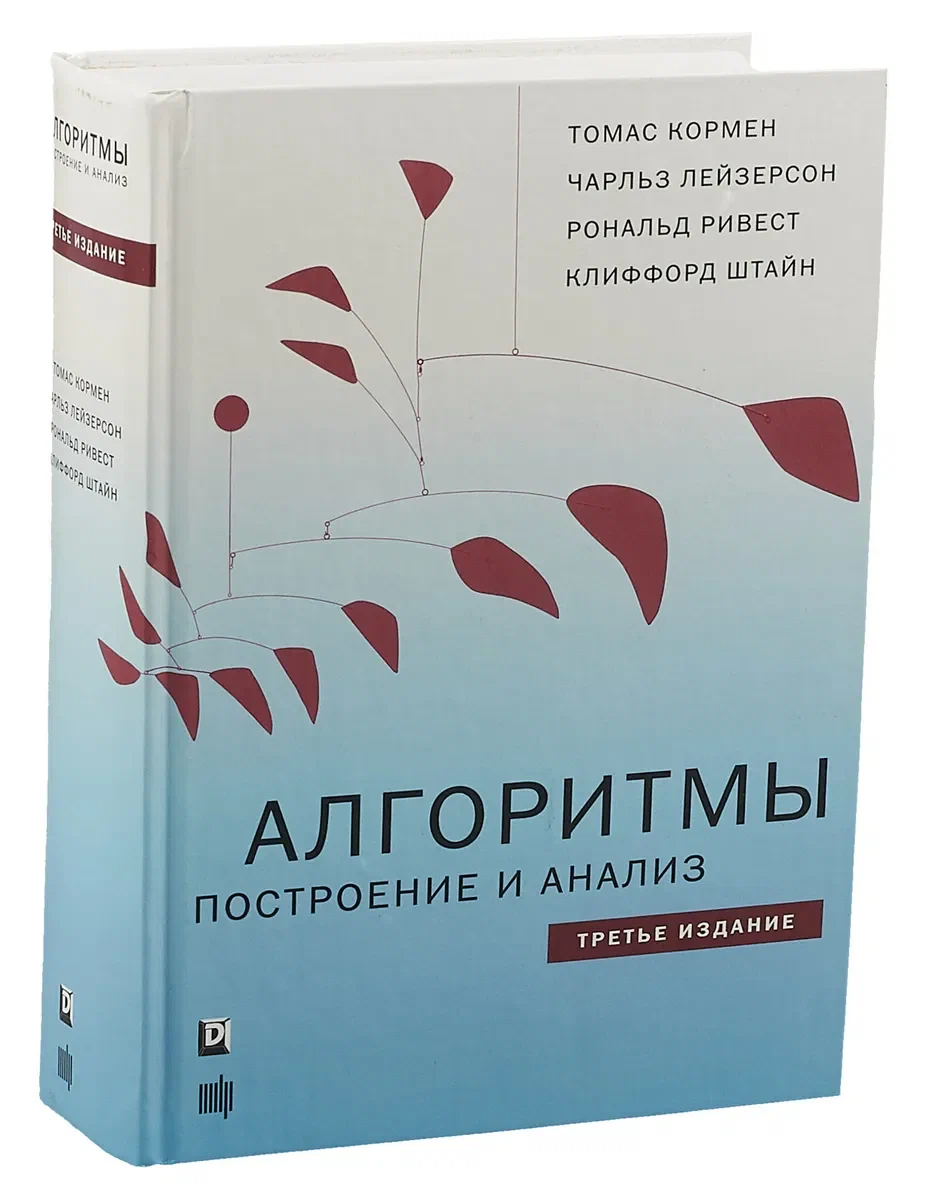
\includegraphics[width=0.4\textwidth]{./../pic/Kormen_3_edition_book_img.png}
<<Алгоритмы. Построение и анализ>>
Томас Кормен
Чарльз Лайзерсон
Рональд Ривест
Клиффорд Штайн.

\begin{block}{Замечание}
	Обязательно купите в бумаге 
	и медленно-медленно читайте...
	Возможно чтение займёт около года -- не пугайтесь. Оно того стоит!
\end{block}

\end{frame}



\section{Базовые понятия}\label{section:base_alg}

\begin{frame}{Алгоритм}
Алгоритм -- это упорядоченная совокупность команд/шагов
для исполнителя (в частности -- вычислительной машины),
обладающая свойствами:
\begin{enumerate}
	\item детерминированность -- что делать на каждом шаге при каждом наборе данных
	\item конечность -- способность завершится для любого набора данных
	\item ... %TODO
\end{enumerate}
 
Свойства алгоритма	
\end{frame}

\begin{frame}{Элементарные операции}
	
\end{frame}

\begin{frame}{Цена деления}
Деление -- сложная и дорогая вычислительная операция.
	
	\begin{block}{Замечание}
	Но не всегда так. 
	Есть "табличный метод",
	есть ПЛИС, видеокарты и т.д.
	
	В которых \textbf{частные} случаи деления происходят быстро.
	\end{block}

\end{frame}

\begin{frame}{Аналоговое деления. Принцип}
 	Ничто не мешает нам исполосовать законы физики для деления...
 	
 	На примере деления на три.
 	
 	\begin{wrapfigure}{L}{0.5\textwidth}
 		\centering
 		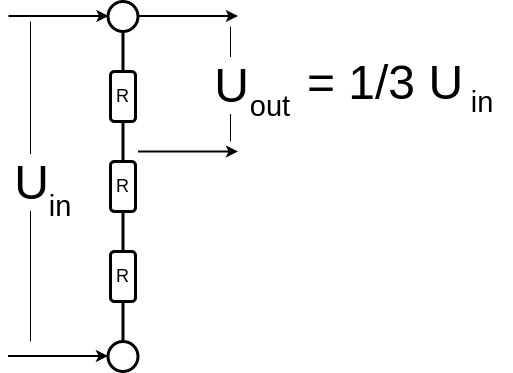
\includegraphics[width=0.5\textwidth]{./../pic/U_division.drawio.png}
 		% \caption{\label{fig:frog1}Пример схемы}
 	\end{wrapfigure}
 	Подаём на вход $U_{in}$ -- количество вольт, равное числу, которое нужно делить на 3.
 	Считываем $U_{out}$ -- делимое.
 	
 	Реальные приборы устроены, конечно, сложнее... Здесь главное понять принцип.

	\вопрос{Достоинства и недостатки подобной конструкции?}

\end{frame}





\begin{frame}{Табличные и полутабличные методы}
	Табличный метод -- мы не вычисляем, а просто создаём большую-пребольшую таблицу (сложения, умножения, деления, возведения в степень и т.д.)
	
	\вопрос{Каковы преимущества и недостатки табличного метода? Когда невозможно использовать табличный методо?}
	
	Полутабличный метод -- мы частично используем таблицу, частично вычисляем.
	
	\вопрос{Можете привести пример? (см пример на слайде №\ref{frame:example_table_method})}.
\end{frame}


\begin{frame}{Сложность алгоритма}
	Сложность алгоритма:
	\begin{enumerate}
		\item Вычислительная сложность -- сколько требуется совершить действий, чтобы алгоритм завершился
		\item Сложность по памяти -- сколько требуется памяти при старте + дополнительно в процессе вычисления, чтобы алгоритм завершился.
	\end{enumerate}
	
	

\end{frame}



\begin{frame}{Сложность $O(g(N))$}
	\footnotesize
	{Главный параметр} (обозначают $N$) -- параметр, наиболее сильно влияющий на вычислительную сложность 
	и/или сложность по памяти.
	
	%\begin{block}{Замечание}
	%	Иногда этих параметров несколько.
	%\end{block}
	
	Функция $f(N)$ имеет порядок сложности $O(g(N))$ 
	если существуют постоянные $c$ и $N_0$ такие что:
	\begin{equation}
	\forall N > N_0  ~\Longrightarrow~ f(N)  \leqslant c \cdot g(N)
	\end{equation}
	
	\termdef{Примеры}
	\begin{itemize}
		\item $f(N)=3 \cdot N^3 + 10 \cdot N^2 + 50$ имеет сложность $O(N^3)$
		\item $f(N)=10000 \cdot N^{10} + 10 \cdot 2^N$ имеет сложность $O(2^N)$
	\end{itemize}

	\begin{block}{Замечание}
		Часто внутри $O$ при решении инженерных задач
		для информативности дополнительно пишут коэффициент $c$.
		
		Тогда для примеров корректнее писать $O(3 \cdot N^3)$ и $O(10 \cdot 2^N)$.
	\end{block}
\end{frame}

\begin{frame}{Сложность $O(g(N))$}
	Вычислительная сложность $O(g(n))$ бывает разная...
	
	\begin{itemize}
		\item $O(1)$ -- скалярная сложность, не зависящая от $N$. Идеальный случай
		\item $O(N^k), k \geqslant 1 $ -- полиномиальная сложность
		\item $O((a+1)^N), a \in \mathbb{N}$ -- экспоненциальная сложность
	\end{itemize}
	
	Например:
	\begin{itemize}
		\item $O(1)$ -- сложность поиска по полю $key$ в конструкции $dict$ языка Python
		\item $O(N)$ -- сложность поиска числа (есть / нет) в неупорядоченном массиве чисел
		\item $O(2^N)$ -- задача Коммивояжера.
	\end{itemize}
\end{frame}

\section{Некотороые примеры}\label{section:examples_1}

\begin{frame}{Поиск элемента в упорядоченном массиве}
	Классическая задачка на собеседованиях :)
	
	Есть упорядоченный массив: от самого малого числа до самого большого. 
	Например $1, 3, 5, 6, 6, ..., 10124, 10345, 12231$. 
	Его длина $N$.
	
	\вопрос{Какова сложность алгоритма поиска <<в лоб>> ?}
	
	\вопрос{Какова сложность оптимального алгоритма поиска ?}
	
\end{frame}


\begin{frame}{Простой полутабличный алгоритм деления}\label{frame:example_table_method}
	Есть некое $N$, не слишком большое, чтобы таблицу $O(N)$ уместить в памяти.
	
	Есть некое плечо $l>>0$. Рассматриваем числа меньшие $l \cdot N$. 
	Можно построить упорядоченный вектор(список) этих чисел:
	\begin{equation}\label{eq:example_table_method_vector_def}
	(B_0=0, B_1 = l, B_2 = 2 \cdot l, ... B_i = i \cdot l, ..., B_N = N \cdot l )
	\end{equation} 
	
	Тогда любой $B_i$ можно вычислить по формуле:
	\begin{equation}\label{eq:example_table_method_B_i}
	\frac{B_i}{c} = \frac{i \cdot l}{c} = i \cdot \frac{l}{c}
	\end{equation}
	
	
 
 	\textbf{Задача.} Число $A < l \cdot N$ нужно разделить на $c<l$.
 	\вопрос{Как решить эту задачу с помощью вектора \eqref{eq:example_table_method_vector_def} и таблицы \eqref{eq:example_table_method_B_i}?}
	
	...
\end{frame}
\begin{frame}
 	...
 	
 	Решение. Можно заметить, что 
 	\begin{equation}
 	\exists i<l, \exists v<l: A = B_i+v
 	\end{equation}
 	Тогда верно:
 	\begin{equation}
 	\frac{A}{c} = \frac{B_i+v}{c} = \frac{B_i}{c} + \frac{v}{c} = i \cdot \frac{l}{c} + \frac{v}{c}
 	\end{equation}
 	
 	C помощью алгоритма поиска можно найти $B_i$ такой что: $B_i <= A < B_{i+1}$ % TODO знак <= на нормальный.
 	
 	Операция умножения дешёвая, операции деления $l$ и $v$ тоже не сильно догорие, 
 	так как $v<l$
 	
 	\дз{Посчитайте сложность этого алгоритма.}
 	
 
		
	
\end{frame}

\section{Базовые принципы}\label{section:base_principles}

\begin{frame}{Жадные алгоритмы}
	Жадные алгоритмы -- это алгоритмы, принимающие оптимальное решение на каждом шаге. Далее -- повторение алгоритма.
	
	\begin{block}{Пример. <<Размен монет>>}
		Монетная система государства Зюзюкия состоит из монет достоинством
		$1, 2, 5, 10, 15, 25$.
		
		Требуется выдать сумму $X$ \textbf{минимальным количеством} монет.
	\end{block}	
	\вопрос{Как решить эту задачу?}
	
\end{frame}

\begin{frame}{Жадные алгоритмы}
	\дз{Разобрать дома классические алгоритмы:}
	\begin{itemize}
		\item Алгоритм Хаффмана
		\item Алгоритм Крускала 
		\item Алгоритм Прима 
		\item Алгоритм Дейкстры
	\end{itemize}
	\дз{Какие из этих алгоритмов жадные?}
\end{frame}


\begin{frame}{Жадные алгоритмы}
	Не для всех задач разумно применять жадные алгоритмы...
	
	
	\begin{itemize}
		\item Оптимальный ход в шахматной партии
		\item Задача Коммивояжёра
		\item \вопрос{ещё примеры?}
		\item \дз{ДЗ.Дома придумать ещё 1-2 примера и записать в тетрадь.}
	\end{itemize}
\end{frame}



% Разделяй и влавствуй

% Жадные алгоритмы

% Таблицы -- это хорошо

% Рекурсии. 

% Паралелизм 
% Map-Reduce принцип


% \section{Базовые проблемы}\label{sections:base_problems}

% \section{Ещё примеры}

\section{Примеры в DSIS}\label{section:examples_2_dsis}

\begin{frame}{Алгоритм поиска серии сериала}
	
	Задача по AntiPiracy
	
	\begin{block}{Задача}
		Существует краулер пиратского видеоконтента.
		
		Необходимо:
		\begin{enumerate}
			\item является ли сериал <<Игрой Пристолов>>?
			\item какой сезон?
			\item какая серия?
			\item если пара (сезон, серия) внутри блок-листа -- дёрнуть REST ручку Роскомнадзора.
		\end{enumerate}
	\end{block}
	
	\textit{Описание алгритма на доске --> }
	
	\дз{Какова вычислительная сложность алгоритма? Сложность алгоритма по памяти}
	
\end{frame}


\begin{frame}{Алгоритм поиска социальной инженерии по поведению}
	
	Задача по UEBA и антифроду
	
	\begin{block}{Задача}
		Существует Online Web банковское приложение.
		
		Требуется определить с полнотой в >70\% и точностью >10\% , находится ли клиент в состоянии социальной инженерии.
	
	\end{block}
	
	\textit{Описание алгритма на доске --> }
	
	\дз{Какова вычислительная сложность алгоритма? Сложность алгоритма по памяти}
	
\end{frame}


\section{Домашнее задание}

\begin{frame}
	\begin{block}{Напоминание}
		Как и ранее, нужно пройтись по всей лекции и записать её тезисно в свою тетрадку конспектом.
		
		Выполнить все задания, отмеченные \дз{этим цветом}.
		
		Пометить на будущее и по возможности понять алгоритмы, отмеченные \внекурса{этим цветом.}
		
		Не ленимся! Иначе зря на DSIS поступали!...
	\end{block}
\end{frame}


\begin{frame}{Разминка}
	

	В Python есть следующие структуры данных:
	set, dict ,tuple, list, str, разные типы данных в \ссылка{https://docs.python.org/3/library/collections.html}{collections}.
	
	
	Какова вычислительная сложность?:
	\begin{itemize}
		\item Поиск элемента;
		\item Вставка элемента;
		\item Удаление элемента.
	\end{itemize}

	Какова цена хранения?
	
	\begin{block}{Замечание.}
		Все вопросы задавать в чате по python, а не по матеше.
	\end{block}
	
	
\end{frame}

\begin{frame}{Умножаем быстро...}
	
	Прочитайте про тривиальный алгоритм умножения и алгоритм Карацубы.
	
	Какова $O(g(n))$ сложность каждого из них?
	
	Как работает алгоритм Карацубы?
	
\end{frame}

\begin{frame}{Сортировки}
	
	Прочитайте про алгоритмы сортировки:
	\begin{enumerate}
		\item Сортировка обезьяны;
		\item Сортировка перемешиванием;
		\item Сортировка вставками;
		\item сортировка Шелла;
		\item Сортировка пузырьком;
		\item Сортировка Хоара;
		\item Гравитационная сортировка (сортировка бусинами);
		\item Сортировка слиянием.
	\end{enumerate}
	
	Какое $O(g(N))$ вычислительной сложности
	имеем 
	в худшем случае; 
	в среднем случае; 
	в наилучшем случае?
	
	Каковы затраты памяти?
	
	
\end{frame}


\begin{frame}{Реализация алгоритма}
	
	Найдите интересный алгоритм, 	\textbf{Застолбите его в чате} и реализуйте его без использования библиотек.
	

	
	\begin{block}{Замечание}
		Если вы используете в качестве языка программирования не компелируемый, а интерпретируемый язык,
		то оберните его в декоратор компилирования в Cи.
		
		Например для языка Python можно использовать \ссылка{https://numba.pydata.org/}{Numba}
	\end{block}
	
	Измерьте скорость работы.
	
	Поделитесь результатами работы с другими ребятами.
	
	Если вы один из первых -- помогите другим ребятам с их алгоритмами.
	
	Чем больше вы поможете -- тем быстрее освоите АиСД.
	
	
\end{frame}


\end{document}